% notations 
% a layer l 
% input x^{(l)}
% output y^{(l)}
%  y^{(l)} = f^{(l)}( W^{(l)} input)
% note that 
% y_i = W_i,: x
% W_ij : x_j -> y_i  
% k is for the class
% l for the layer 


%%%%%%% to define layers math notations 
\newcommand{\inp}{\ensuremath{\x}}
\newcommand{\outp}{\ensuremath{\seq{y}}}
\newcommand{\lid}[1]{\ensuremath{^{(#1)}}}

%%%%%%% data and loss
\newcommand{\dlta}{\ensuremath{\delta}} % gradient component of pre-activation
\newcommand{\vdlta}{\ensuremath{\seq{\delta}}} % gradient vector of pre-activation

\colorlet{darkgreen}{green!50!black}


%% draw one layer 
\newcommand{\layer}{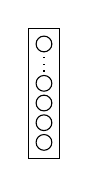
\begin{tikzpicture}[baseline=0.5ex]%
    \foreach \y in {0.25,0.5,...,1}{ 
      \draw (0,\y) circle  (0.1);%
    }
    \draw[dotted] (0.0, 1.15) -- (0.0,1.35); 
    \draw (0,1.5) circle (0.1);
    \draw (-0.2,0.05) rectangle (0.2,1.7);
\end{tikzpicture}}

%% draw connection
\newcommand{\connection}{\begin{tikzpicture}[baseline=0.5ex]%
    \draw[->] (0,0.85) -- (1.0,0.85);
\end{tikzpicture}}
%% dotted connection
\newcommand{\dotted}{\begin{tikzpicture}[baseline=0.5ex]%
    \draw[dotted,thick] (0,0.85) -- (0.5,0.85);%
\end{tikzpicture}}

\newcommand{\raiseW}{2ex}
% for computational graph
\newcommand{\vnode}{\node}
\newcommand{\funnode}{\node[minimum size=1.5,rectangle,draw=green,fill=green!20]}
\newcommand{\inlinefnode}[1]{\raisebox{-5pt}{\tikz{\funnode {#1}}}}



\newcommand{\justunder}{0.5cm}
\newcommand{\largeurUn}{0.8}
\newcommand{\largeurDeux}{0.7}
\setbeamercolor{postit}{fg=black,bg=red!30}
\setbeamercolor{mygreen}{fg=black,bg=green!20}
\setbeamercolor{myred}{fg=black,bg=red!20}
\setbeamercolor{darkpostit}{fg=black,bg=red!64}
\setbeamercolor{text}{fg=black,bg=red!10}


%%%%%%%%%% NNet for NLP
%% draw one layer  
\newcommand{\wemb}{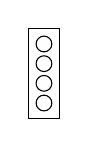
\begin{tikzpicture}[baseline=0.5ex]%
    \foreach \y in {0.25,0.5,...,1}{ 
      \draw (0,\y) circle  (0.1);%
    }
    \draw (-0.2,0.05) rectangle (0.2,1.2);
\end{tikzpicture}}

\newcommand{\worddim}{\ensuremath{K}} % dimension of the word embeddings
\newcommand{\wvector}{\ensuremath{\vct{v}}} % word vector
\newcommand{\wmatrix}{\ensuremath{\vct{R}}} % word matrix
\newcommand{\dvector}{\ensuremath{\vct{d}}} % document vector

